% Mit folgendem Header kann ich wahlweise 'latex bla.tex', oder 'pdflatex
% bla.tex' laufen lassen. Es wird dann eine dvi bzw. pdf Datei erzeugt. Die
% Bilder, die mit includegraphics importiert werden, werden ohne Dateiendung
% angegeben. Latex sucht sich dann entweder ein .eps bzw. .pdf/.png/.jpg File
% heraus...
%
%(http://www.techfak.uni-bielefeld.de/ags/ni/lectures/internstuff/howto/howto-la
%tex/howto-pdflatex.html)
\newif\ifpdf \ifx\pdfoutput\undefined
\pdffalse % we are not running pdflatex
\else
\pdfoutput=1 % we are running pdflatex
\pdfcompresslevel=9 % compression level for text and image;
\pdftrue \fi

\documentclass[12pt, headsepline]{scrreprt}
\usepackage[ngerman]{babel}

\ifpdf
  \usepackage[pdftex,xdvi]{graphicx}
  \usepackage[pdftex]{hyperref}         % option [colorlinks] erzeugt farbige Links statt

  \pdfinfo{
     /Title    (Abschlussbericht Muminav)
     /Author   (Michael Gl�ssel, Matthias Erche, J�rg K�ster)
     /Subject  ()
     /Keywords (tu-berlin, open source, java)
  }
  \usepackage[pdftex]{color}            % farbige Umrandungen
\else
  \usepackage[dvips,xdvi]{graphicx}
  \usepackage[colorlinks]{hyperref}
  \usepackage{color}
\fi

\usepackage[automark,headsepline,plainheadsepline]{scrpage2}
\pagestyle{scrheadings}
%\ohead[\pagemark]{\pagemark}
\ohead[\headmark]{\headmark} \chead{\empty}


% ersetzt, s. o.
% \usepackage{color}                    % um den Text auch farbig zu gestalten
% \usepackage[dvips]{graphicx}          % zum Einbinden von Grafiken, [<TREIBER>]

%\usepackage{subfigure}                  % mehrere figures in einem floating object
\usepackage[latin1]{inputenc}           % f�r Umlaute
\usepackage{textcomp}                   % fuer Sonderzeichen wie <Grad Celsius>
% \usepackage{hyperref}                 % zum Einbinden von Querverweisen in pdf (als letztes
                                        % auffuehren!)
%\graphicspath{{figs/}}               % jetzt muss man nicht jedesmal den Pfad angeben

\usepackage{array}

\DeclareRobustCommand{\trademark}{\ensuremath{^{\mathrm{TM}}}}


\title{Abschlussbericht \\ Muminav}

\author{
  Open-Source-Softwareprojekt\\
  Sommersemester 2002\\
  Technische Universit�t Berlin \\ \\
  \normalsize Michael Gl�ssel \\
  \normalsize Matthias Erche \\
  \normalsize J�rg K�ster\\
}

\date{\today}

\begin{document}                        % here begins the actual document body
%\maketitle                             % this actually creates the title block




\vspace*{\stretch{1}} \rule{\linewidth}{1mm}

\begin{flushright}
    \thispagestyle{empty}
    {\Large \textbf{Abschlu�bericht}\\}
 %   {\Huge \textbf{Muminav}\\}
\begin{figure}[htbp]
    \begin{flushright}
        
\includegraphics[width=10cm]{figs/logo}
    \end{flushright}
\end{figure}
    \vspace{0.1cm}
    %\large



\begin{minipage}[b]{13cm}
\begin{raggedleft}
    Im Rahmen der Veranstaltung:\\
    Dezentrale Systementwicklung am Beispiel GNU/LINUX\\
    an der TU-Berlin --
    Sommersemester 2002\\
\end{raggedleft}
\end{minipage}
%\hspace*{21mm}
%\begin{minipage}[b]{\linewidth}
\begin{minipage}[t]{2cm}

\includegraphics[height=1.5cm]{figs/tulogo}
\end{minipage}





    }

\end{flushright}


\rule{\linewidth}{1mm}





\vspace*{\stretch{2}}
\begin{center}
\large \textsc{Michael Gl\"assel, Matthias Erche, J�rg K�ster} \\
{\normalsize Betreuung: \textsc{Steffen Evers}}\\
\vspace{0.7cm} \today\\
%\begin{figure}[htbp]
%       \centering
%        
\includegraphics[width=1.5cm]{figs/tulogo}
%\end{figure}
\end{center}


\begin{abstract}
\textbf{Zusammenfassung} blah \ldots
\end{abstract}

\tableofcontents

%--------------------------------------------------------------------
\chapter{Einleitung}

\section{Der Projektkontext}

F�r eine moderne mathematische Ausbildung von Ingenieuren ist
mittlerweile nicht nur der Umfang des erworbenen Wissens wichtig,
vielmehr muss neben der reinen Vermittlung von Fachwissen Wert auf
das Verst�ndnis von Zusammenh�ngen gelegt werden. Heutzutage ist
es durch immer schneller anwachsendes Wissen mehr denn je
erforderlich, dass sich Ingenieure einem st�ndigen Lernprozess
unterziehen. Die Unterst�tzung dieses Prozesses durch zeitgem��e,
multimediale Technologien ist dabei nur folgerichtig. Es werden
neue M�glichkeiten er�ffnet, Zusammenh�nge darzustellen, die
Kommunikation zwischen Dozent und Lernenden und das selbstst�ndige
Aneignen von Lehrstoff zu f�rdern.

So haben sich vier deutsche Universit�ten im Projekt \glqq
Multimediale Mathematikausbildung f�r Ingenieure\grqq\
\footnote{kurz: \textsc{Mumie}} \cite{Mumie} zusammengeschlossen,
um die Idee von einer \glqq modernen Mathematikausbildung\grqq\ zu
verwirklichen.

\subsection{Dezentrale Systementwicklung am Beispiel GNU/Linux}

Das Projekt \glqq Mumie\grqq\ soll nach aktuellem Stand unter
einer Open Source-Lizenz entwickelt und ver�ffentlicht werden. Die
Zusammenarbeit zwischen den Universit�ten impliziert eine
dezentrale Entwicklung, an der auch das Projekt \glqq
\textsc{MumiNav}\grqq\ beteiligt ist. Das bei der Entwicklung
entstehende Produkt wird nicht zur \glqq Insell�sung\grqq\ , da es
in ein
bestehendes Projekt integriert wird.\\
 Eine Aussicht auf die
Verwendung schon existierender Software besteht unter Umst�nden
bei der Realisierung der Datenschnittstelle. So gehen erste
�berlegungen in die Richtung, schon bestehende XML-Software zu
verwenden, um die vom Server �bertragenen Daten auszuwerten.

\subsection{Das Projekt Mumie}

Das Projekt wird vom Bundesministerium f�r Bildung und Forschung
gef�rdert. Es soll eine WWW-basierte, modulare Umgebung entwickelt
werden, welche sowohl den Lernenden als auch Dozenten eine
grafisch ansprechende und leicht zu bedienende Oberfl�che bietet.
So wird einerseits durch die Visualisierung mathematischer Inhalte
und dem interaktiven Umgang mit der Mathematik die Motivation
gef�rdert. Zus�tzlich werden einige lehr-- und lernbegleitende
Tools angeboten:

\begin{itemize}
\raggedright
\item Darstellung mathematischer Inhalte mit interaktiver
Multimedia-Unterst�tzung
\item Stoffnachbereitung, Wiederholungsunterst�tzung angeleitete und kommen\-tier\-te
�bungs\-auf\-gaben
\item Selbstkontrolle durch individuelle
Testumgebungen
\item Einf�hrung in mathematische Standardsoftwarepakete
\item individuelles Trainingscenter weiterf�hrender
Inhalte
\item Informationsplattform in der und vile und in die der es auch
noch kein wer, was, wie, wo
\item Kommunikations-- und
Austauschangebote
\end{itemize}

Die urspr�ngliche Idee hierbei ist, mathematische Inhalte
darzustellen. Die Umgebung soll allerdings so gestaltet werden,
dass sie auch in anderen Disziplinen genutzt werden kann. Weitere
Schwerpunkte liegen auf der Individualisierung der Oberfl�che und
einer intelligenten Benutzerf�hrung, die verhindert, dass man in
der inhaltlichen F�lle des Gesamtangebotes die �bersicht verliert.

\section{Ziele}

Der Dozent soll die M�glichkeit haben, aus einer Auswahl an
Elementen \footnote{Motivation, Definition, Theorem, Lemma,
Algorithmus, Anwendung}, die in einer Datenbank gespeichert sind,
die Zusammenstellung f�r einen Kurs zu erstellen. Dies soll durch
einfaches Ziehen und Ablegen von Elementsymbolen auf einer
Zeichenfl�che erfolgen. Zusammenh�nge zwischen Elementen werden
dabei durch Verbindungslinien dargestellt, die der Verfasser
positionieren kann. Zus�tzlich kann es zu den Elementen
Subelemente \footnote{Herleitung, Beweis, Motivation, Bemerkung,
Historisches, Visualisierung, Beispiel, Tabelle} geben. Es
entsteht durch die Zusammenstellung eine Repr�sentation der
mathematischen Zusammenh�nge mittels eines gerichteten Graphen.
Der Dozent kann zur Darstellung des Kursverlaufes eine Art \glqq
roten Faden\grqq\ festlegen, der allerdings nicht entlang der
angelegten Verbindungen laufen muss \footnote{Aktueller Stand,
�nderungen m�glich}.

Die Aufgabe f�r das Projekt \textsc{MumiNav} besteht darin, dieses
vorgegebene Netz mit Hilfe eines Java-Applets in einem
Navigationsframe darzustellen und somit den Zugriff auf die
Inhalte zu erm�glichen. Die Darstellung der Elemente erfolgt durch
unterschiedlich farbige, leicht dreidimensional angedeutete
K�sten. Subelemente werden nach vorgeschriebenen Regeln an diesen
K�sten angeordnet und sind standardm��ig nicht mit
Unterscheidungsmerkmalen versehen.

\begin{figure}[htbp]
    \centering%
%   \setcapwidth[c]{12cm}%
    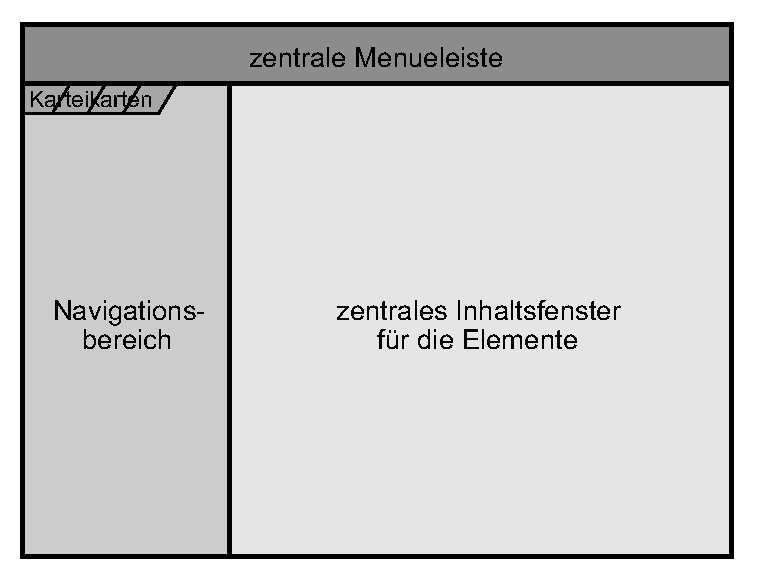
\includegraphics[width=8cm]{figs/haupframe}
    \captionbelow{Layout der Hauptansicht}
    \label{FIG:Hauptansicht}
\end{figure}

Die Abbildung des logischen Netzes geschieht, wie vorher
beschrieben, durch Verbindungslinien zwischen den Elementsymbolen.
Es wird ein \glqq roter Faden\grqq\ entsprechend der linearen
Anordnung der Kursinhalte gelegt.

\begin{figure}[htbp]
    \centering%
%   \setcapwidth[c]{12cm}%
    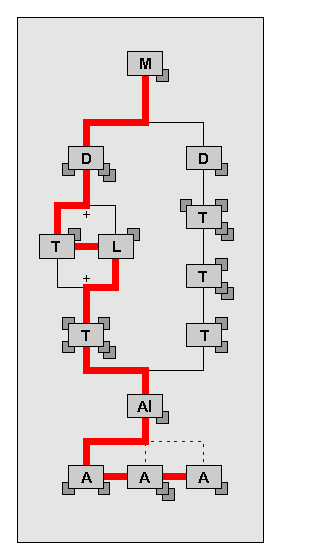
\includegraphics[height=7cm]{figs/navinetz}
    \captionbelow{Kurspfade und roter Faden}
    \label{FIG:roterFaden}
\end{figure}



Die Darstellung soll auf mehrere Maus-Aktionen reagieren. Wird die
Maus �ber ein Element bewegt, soll dieses vergr��ert dargestellt
werden und die Subelemente werden unterscheidbar durch
Beschriftung. Bei Klick mit der linken Maustaste soll der Inhalt
des jeweiligen (Sub-)Elementes im zentralen Inhaltsfenster
dargestellt werden. Dieselbe Aktion auf der mittleren Maustaste
f�hrt zu einem �ffnen des Inhalts in einem externen Fenster und
schlie�lich ist es zuk�nftig vorgesehen, mit der rechten Maustaste
eine Liste von Optionen anzubieten.

\begin{figure}[htbp]
    \centering%
%   \setcapwidth[c]{12cm}%
    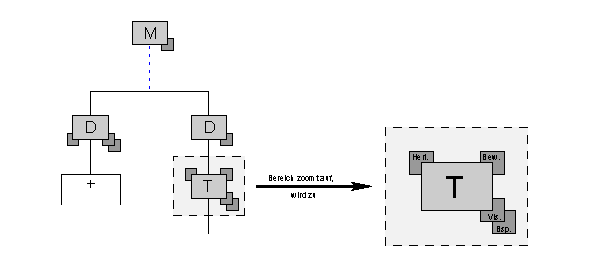
\includegraphics[width=10cm]{figs/zoom_element}
    \captionbelow{Detailansicht bei Zoom}
    \label{FIG:zoomElement}
\end{figure}


\chapter{Organisation des Gesamtprojekts}

An \textsc{Muminav} haben im Rahmen der Veranstaltung
\emph{Dezentrale Systementwicklung am Beispiel GNU/LINUX}
mitgewirkt: J�rg K�ster, Matthias Erche und Michael Gl�ssel, alles
Studenten der TU-Berlin im Fach Informatik.

\section{Meilensteine}

Die Termin- und Sachzielverfolgung wurde mit Hilfe von 4
Meilensteinen sichergestellt.

\begin{itemize}
\item \textbf{8.\ Mai} Festlegung auf eine Projektaufgabe
\item \textbf{29.\ Mai} Bestandsaufnahme von relevanten Projekten
\item \textbf{19.\ Juni} Vorlage des L�sungskonzept
\item \textbf{1.\ Oktober} Zwischenbilanz und Prototyp
\end{itemize}



\section{Workshops}

Beim Workshop, der am 10.\ Juli stattfand, ging es um die
Nachbearbeitung, Analyse und Erg�nzung der gesammelten
Erfahrungen. Dazu wurden Gastredner eingeladen, die sich seit
l�ngerer Zeit im Bereich Open Source (Softwareentwicklung) bet�tigen und die mit ihrem Wissen
dazu beitragen konnten, die pers�nlichen Erfahrungen der Teilnehmer
in einem allgemeineren und objektiverem Zusammenhang zu sehen.


\section{Gruppenaufteilung}


Die Entwicklungs- und Implementierungsarbeit hat sich wie folgt
aufgeteilt:

\begin{itemize}
    \item \textbf{Matthias Erche} Betreuung der Projektwebseite, Projekt Organisation, Entwurf des Datenaustauschformates, Programmierung der XML Verarbeitung, Dokumentation
    \item \textbf{J�rg K�ster} �berarbeitung der Zeichenengine, Zoomfunktionalit�t, Entwurf diverser (Zeichen-) Algorithmen, Skinprogrammierung, Dokumentation

    \item \textbf{Michael Gl�ssel} Umsetzung des Grundger�sts, Eventhandling, Projekt Organisation, Tooltips, Zeichenalgorithmen
\end{itemize}

Ausserdem haben sich alle drei bei der Konzeptentwicklung, der Recherche nach relevanten Projekten und dem Schreiben des Abschlussberichtes beteiligt. Zu jedem der ersten drei Meilensteine hat jeweils ein Gruppenmitglied einen Vortrag gehalten.


\chapter{Muminav}

\section{Lizenz}

Vorgabe war, die gesamte Entwicklungsarbeit als Open Source
Projekt durchzuf�hren. Dies schlie�t ein, die
Projektergebnisse unter einer Open Source Lizenz zu ver�ffentlichen.\\
Da wir unser Projekt in Zusammenarbeit mit der Mumie-Gruppe
entwickeln, mussten wir uns im Vorfeld mit Ihnen auf eine Open
Source Lizenz verst�ndigen, welche in das Gesamtprojekt Mumie
integrierbar ist.\\
Die GPL \cite{GPL} (GNU General Public License)



LGPL \cite{OpenSourceLicences},\cite{LGPL}.

\section{Entwicklungsumgebung}
\subsection{Projekthoster}
\subsection{Enwicklungswerkzeuge} Ant \cite{Ant2002}, JBuilder \cite{BerliOS}

\chapter{Beurteilung des Projekts}

\section{Diskussion des Status quo}

\section{Einsatzf�higkeit}

\textsc{Muminav} wurde als hoch spezialisierte Softwarekomponente
f�r den Einsatz im Gesamtprojekt \textsc{Mumie} ins Leben gerufen.
Nichts desto trotz haben wir gro�en Wert darauf gelegt, die
Software so allgemein wie m�glich zu gestalten damit sie f�r
m�glichst viele andere Open-Source-Projekte interessant wird.
Letztendlich wurde, durch den Einsatz von Skins und XML als
Datenformat, aus der Aufgabe, ein Java-Applet zu programmieren,
welches Navigationsnetze f�r Mathematische Kurse im Internet
dynamisch erzeugt, ein Softwaremodul, welches f�r die Darstellung
jeglicher graphischer Darstellungen geeignet ist. Zum Beispiel
lie�en sich leicht Skins erstellen, mit denen man Flowcharts, E/R
Diagramme oder sogar UML darstellen kann.\\
Zus�tzlich ist die Software so ausgelegt, dass sie nicht auf
Applets beschr�nkt ist. Durch das Packaging in ein
Java-Swing-Panel l�sst es sich genau so gut in eine
Java-application einbauen.

\section{Ausblick}

F�r die Zukunft des Projekts haben wir uns vorgestellt, den
Abstraktionsgrad weiter zu steigern, damit es immer leichter wird,
seine eigenen Skins zu entwerfen.\\
Angedacht ist auch ein einfacher Skin-Editor, mit dem man sich
bequem per Maus seine eigenen Skins entwerfen kann.\\
Wir werden auch versuchen eine kleine Community zum leben zu
erwecken, die gegenseitig Skins austauscht. Dabei k�nnte man die
\textsc{Muminav}-Homepage zu einem �ffentlich zug�nglichen
Skin-Archiv erweitern, in das jeder seine Skin einbringen und bei
Bedarf von der Kreativit�t anderer profitieren kann.

Was eigentlich gar nicht erw�hnt werden m�sste: Das
\textsc{Muminav}, wie auch jedes andere Open-Source-Projekt, ist
mit der Fertigstellung der ersten Version nicht abgeschlossen.
Vielmehr wird es, solange es aus der Open-Source-Community
Interesse und Anregungen gibt, sich weiterentwickeln. Sei es durch
entdeckte Bugs oder Vorschl�ge f�r neue Features, die durch uns
oder Mitglieder aus der Open-Source-Community in das Projekt
einflie�en. 

%--------------------------------------------------------------------


\bibliographystyle{bibstyle} % mit custom-bib erzeugter individueller Bibliographie-Style !!
\bibliography{bibliographie}


\end{document}
